\documentclass[12pt,a4paper,utf8]{ctexart}
\usepackage{graphicx}
\usepackage{amsmath}
\usepackage{amssymb}
\usepackage{subfig}
\usepackage{cite}
\usepackage[ntheorem]{empheq}
\usepackage{enumitem}
\usepackage{fullpage}
\usepackage{cleveref}
\usepackage{cellspace}
\usepackage{listings}
\usepackage{color}
\usepackage{algorithm}  
\usepackage{algorithmicx}  
\usepackage{algpseudocode}  
\definecolor{gray}{rgb}{0.5,0.5,0.5}
\definecolor{dkgreen}{rgb}{.068,.578,.068}
\definecolor{dkpurple}{rgb}{.320,.064,.680}
\usepackage{lipsum}

\makeatletter
\newenvironment{breakablealgorithm}
  {% \begin{breakablealgorithm}
   \begin{center}
     \refstepcounter{algorithm}% New algorithm
     \hrule height.8pt depth0pt \kern2pt% \@fs@pre for \@fs@ruled
     \renewcommand{\caption}[2][\relax]{% Make a new \caption
       {\raggedright\textbf{\ALG@name~\thealgorithm} ##2\par}%
       \ifx\relax##1\relax % #1 is \relax
         \addcontentsline{loa}{algorithm}{\protect\numberline{\thealgorithm}##2}%
       \else % #1 is not \relax
         \addcontentsline{loa}{algorithm}{\protect\numberline{\thealgorithm}##1}%
       \fi
       \kern2pt\hrule\kern2pt
     }
  }{% \end{breakablealgorithm}
     \kern2pt\hrule\relax% \@fs@post for \@fs@ruled
   \end{center}
  }
\makeatother

\floatname{algorithm}{算法}  
\renewcommand{\algorithmicrequire}{\textbf{输入:}}  
\renewcommand{\algorithmicensure}{\textbf{输出:}}  

% set Matlab styles
\lstset{
   language=Matlab,
   keywords={break,case,catch,continue,else,elseif,end,for,function,
      global,if,otherwise,persistent,return,switch,try,while},
   basicstyle=\ttfamily,
   keywordstyle=\color{blue}\bfseries,
   commentstyle=\color{dkgreen},
   stringstyle=\color{dkpurple},
   backgroundcolor=\color{white},
   tabsize=4,
   showspaces=false,
   showstringspaces=false
}

\begin{document}
\CJKfamily{zhkai}	


\begin{center}
\textbf{计算方法 作业二}\\
\textbf{姓名 ~范文~~~~~~~~ 学号 ~PB18111679~~~~~~ 日期 2021.6.3}\\
\end{center}

\begin{center}
\fbox{
\begin{minipage}{40em}
\vspace{5cm}
\hspace{20cm}
\end{minipage}}
\end{center}
\vspace{1cm}

\paragraph{实验环境}
\subparagraph{硬件配置}
        8个Intel(R) Core(TM) i5-8250U核,内存8G,交换区8G
\subparagraph{操作系统}
        ubuntu 20.04,内核版本为5.4.0-72-generic
\subparagraph{Matlab}
        MATLAB R2016b 

\begin{enumerate}
\item[第一题] \textbf{三次样条插值法}

    \begin{itemize}
    \item [(a)] \textbf{第二类边界条件中线性方程组的推导}
    \par
    由课本(1.22)式可知,在每个区间$[x_i,x_{i+1}]$内,插值函数的表达式为
    \begin{equation}
        \begin{aligned}
        S(x) = \frac{ (x_{i+1} - x)^3 M_i + (x - x_i)^3 M_{i+1} }{6 h_i}  
            +  \frac{ (x_{i+1} - x) y_i + (x - x_i) y_{i+1} }{ h_i} \\
            - \frac{h_i}{6}( (x_{i+1} - x)M_i + (x - x_i)M_{i+1} ) \label{S}
        \end{aligned}
    \end{equation}

    \par
    因此,在每个区间$[x_i,x_{i+1}]$内,插值函数的导数为
    \begin{equation}
        \begin{aligned}
        S(x) &= \frac{ -3(x_{i+1} - x)^2 M_i - 3(x - x_i)^2 M_{i+1} }{6 h_i}  
            +  \frac{ y_{i+1} - y_i }{ h_i} 
            - \frac{h_i}{6}( ( M_{i+1} - M_i ) \\
            &=  \frac{ -(x_{i+1} - x)^2 M_i - (x - x_i)^2 M_{i+1} }{2 h_i}
            +  f[x_i,x_{i+1}] - \frac{h_i}{6}( ( M_{i+1} - M_i ) \label{S'}
        \end{aligned}
    \end{equation}
    \par
    设$f'(x_0) = m_0,f'(x_n) = m_n$,由此可得
    \begin{equation}
      \begin{aligned}
      S'(x_0) &= -\frac{h_0 M_0}{2} + f[x_0,x_1] + \frac{h_0M_0}{6} - \frac{h_0M_1}{6} \\
      &= f[x_0,x_1] - \frac{h_0M_0}{3} - \frac{h_0M_1}{6} 
       = m_0 \label{S'(x_0)}
      \end{aligned}
    \end{equation}
    \par
    即有
    \begin{equation}
      \begin{aligned}
      2 M_0 + M_1 = \frac{6}{h_0}(f[x_0,x_1] - m_0) = d_0
      \end{aligned}
    \end{equation}

    \par
    同理可知
    \begin{equation}
      \begin{aligned}
      S'(x_n) &= f[x_{n-1},x_n] + \frac{h_{n-1}M_{n-1}}{6} + \frac{h_{n-1}M_{n}}{3} = m_n \label{S'(x_0)}
      \end{aligned}
    \end{equation}
    \par
    即有
    \begin{equation}
      \begin{aligned}
      M_{n-1} + 2M_n = \frac{6}{h_{n-1}}(m_n - f[x_{n-1},x_n]) = d_n
      \end{aligned}
    \end{equation}
    \par
    因此,满足的线性方程组为
    \begin{equation}
      \begin{aligned}
      \begin{pmatrix}
        2 & 1 \\
        \mu_1 & 2     & \lambda_1 \\
              & \mu_2 & 2 & \lambda_2 \\
              &       &   & \ddots \\ 
              &       &   & \mu_{n-1} & 2 & \lambda{n-1} \\
              &       &      &     & 1 & 2 
      \end{pmatrix}
      \begin{pmatrix}
        M_0 \\
        M_1 \\
        M_2 \\
        \vdots \\
        M_{n-1} \\
        M_{n}
      \end{pmatrix} = 
      \begin{pmatrix}
        d_0 \\
        d_1 \\
        d_2 \\
        \vdots \\
        d_{n-1} \\
        d_{n}
      \end{pmatrix}
      \end{aligned}
    \end{equation}

    \item [(b)] \textbf{三次样条插值(边界条件2)的逐点误差}
    我使用MATLAB计算(7)中的线性方程组,得到了[-1,1]内 $2^4$个均匀划分的子区间的插值函数.并计算这个插值函数与原函数在[-1,1]之间的2000个均匀划分的点上的逐点误差如图1所示.

    \begin{figure}[htbp]
      \centering
      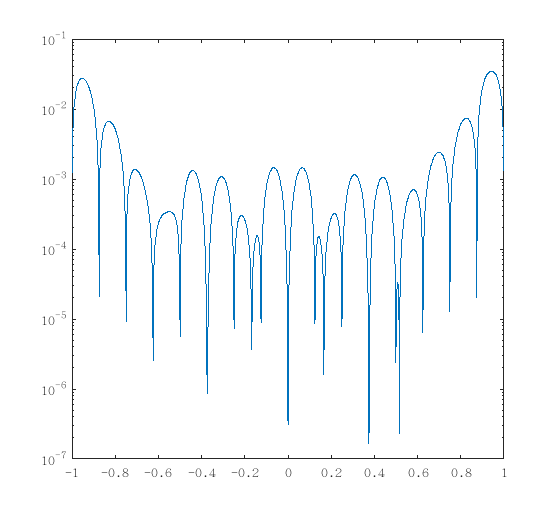
\includegraphics[scale=0.7]{pictures/p1_2.png}
      \caption{\small{三次样条插值(边界条件2)的逐点误差}} %图1
    \end{figure}

    \item [(c)] \textbf{三次样条插值(边界条件2)的最大误差}
    还是利用(b)中的代码,计算
    $\{2^4,2^5,\\ 2^6,2^7,2^8,2^9,2^{10}\}$
    每一组均匀划分的点的逐点误差的最大值,
    得到了最大误差随区间数$n$的变化如图2所示.

    \begin{figure}[htbp]
      \centering
      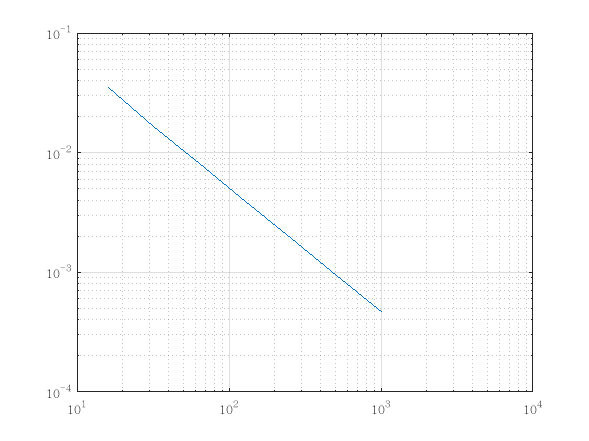
\includegraphics[scale=0.7]{pictures/p1_3.png}
      \caption{\small{三次样条插值(边界条件2)的最大误差随区间数$n$的变化}} %图2
    \end{figure}
    
    \par
    而求三次样条插值(边界条件2)的MATLAB代码如下所示.
    \begin{lstlisting}[frame=single]
% implementing spline with boundary condition 2
% @F: the function to approximate in [-1,1]
% @n_list: stores the number of intervals in [-1,1]
% @k: number of testing points in [-1,1]
% @opt: 0: plot the semilogy of errors on each point
%       1: plot the semilogy of max error in each case 
function spline_boundary_condition_2(F,n_list,k,opt)
    
    % max_errors stores the max error 
    % of testing points on each n
    [~,n_list_col] = size(n_list);
    max_errors = zeros(1,n_list_col);
    
    % get the max_error on each n
    for index = 1 : n_list_col
    
        n = n_list(index);
        % get the info of intervals
        % x marks interval end points
        % h marks interval length
        % df marks the diff of the function value 
        % at the start and the end of the interval
        x = linspace(-1, 1, n + 1);
        f = F(x);
        h = diff(x);
        df = diff(f);
    
        % lambda and mu are parameters in A
        lambda = h(2:n) ./ ( h(2:n) + h(1:n - 1) );
        mu = 1 - lambda;
    
        % d is on LHS of the linear equation
        % get d(1) ~ d(n-1)
        d = 6 * ( df(2:n) ./ h(2:n) - df(1:n - 1) ... 
            ./ h(1:n-1) ) ./ ( h(1:n-1) + h(2:n) );
    
        % for boundary condition 2,
        % get d(0) and d(n)
        m_0 = 0;
        m_n = 0;
    
        d = d.';
        d_0 = 6 * ( df(1) / h(1) - m_0 ) / h(1);
        d_n = 6 * (m_n - df(n) / h(n) ) / h(n);
        d = [d_0; d; d_n];
    
        % A is the parameters of this linear equation
        % get A
        A = 2 * eye(n+1);
        A(1,2) = 1;
        A(n+1,n) = 1;
        for i = 2 : n - 1
            A(i,i-1) = mu(i);
            A(i,i+1) = lambda(i);
        end
    
        % get M where AM = d
        M = A \ d;
        errors = get_errors(F,x,h,M,k);
        % for opt = 0, now k = 2^4
        % plot the errors of approximation 
        % on each testing point
        if(index == 1 && opt == 0)
            test_x = linspace(-1,1,k);
            semilogy(test_x,errors);
        end
        max_errors(index) = max(abs(errors));
    end
    
    % for opt = 1,
    % plot the max error of each interpolation
    if(opt == 1)
        loglog(n_list,max_errors);
        grid on;
    end
end

% get the error on each testing point
% @F: the function in [-1,1]
% @x: the points of each interval in [-1,1]
% @h: the length of each interval
% @M: the second order derivative
%   on the point of each interval
% @k: number of testing points
function errors = get_errors(F,x,h,M,k)
    test_x = linspace(-1,1,k);
    errors = test_x;
    i = 1;
    for j = 1 : k
        % get the interval that the testing point is in
        x_0 = test_x(j);
        while( x_0 > x(i+1) )
            i = i + 1;
        end
        gap_up = x(i+1) - x_0;
        gap_down = x_0 - x(i);
        % S is the approximate value
        S = (gap_up^3 * M(i) + gap_down^3 * M(i+1))...
            / (6*h(i)) + ...
            (gap_up * F(x(i)) + gap_down * F(x(i+1)))...
             / h(i) - ...
            h(i)*(gap_up * M(i) + gap_down * M(i+1))/6;
        errors(j) = abs( F(x_0) - S );
    end
end
      
    \end{lstlisting}

    \item [(d)] \textbf{第三类边界条件中线性方程组的推导}
    \par
    由周期性条件知,$m_0 = m_n$且$M_0 = M_n$,则由(3)(5)有
    \begin{equation}
      \begin{aligned}
      f[x_0,x_1] - \frac{h_0M_0}{3} - \frac{h_0M_1}{6} &= 
      f[x_{n-1},x_n] + \frac{h_{n-1}M_{n-1}}{6} + \frac{h_{n-1}M_{n}}{3}
      \end{aligned}
    \end{equation}
    \par
    即可化为
    \begin{equation}
      \begin{aligned}
     2(h_0 + h_{n-1})M_0 + h_{n-1}M_{n-1} + h_0M_1 &=   
     6f[x_0,x_1] + 6f[x_{n-1},x_n] &= d_0
      \end{aligned}
    \end{equation}
    \par
    因此,可以得到线性方程组
    \begin{equation}
      \begin{aligned}
      \begin{pmatrix}
      2(h_0 + h_{n-1}) & h_0 & &   &   & h_{n-1} \\ 
      \mu_1 & 2     & \lambda_1 \\
             & \mu_2  & 2   & \lambda_2 \\
              &       & \ddots \\ 
            &     &  &  \mu_{n-2} & 2 & \lambda_{n-2} \\
      \lambda_{n-1}      &     &  &   & \mu_{n-1} & 2 \\
      \end{pmatrix}
      \begin{pmatrix}
        M_0 \\
        M_1 \\
        M_2 \\
        \vdots \\
        M_{n-2} \\
        M_{n-1}
      \end{pmatrix} = 
      \begin{pmatrix}
        d_0 \\
        d_1 \\
        d_2 \\
        \vdots \\
        d_{n-2} \\
        d_{n-1}
      \end{pmatrix}
      \end{aligned}
    \end{equation}

    类似地,写出三次样条插值(边界条件3)的MATLAB程序,分别计算当区间数$n = 2^4$时,2000个均匀测试点上的逐点误差以及$n = \{2^4,2^5,2^6,2^7,2^8,2^9,2^{10}\}$时每一组均匀划分的点的逐点误差的最大值,分别得到图3和图4.

    \begin{figure}[htbp]
      \centering
      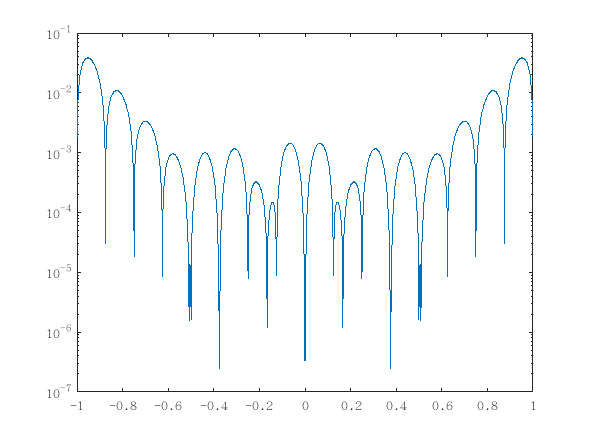
\includegraphics[scale=0.7]{pictures/p1_4_2.png}
      \caption{\small{三次样条插值(边界条件3)的逐点误差}} %图1
    \end{figure}

    \begin{figure}[htbp]
      \centering
      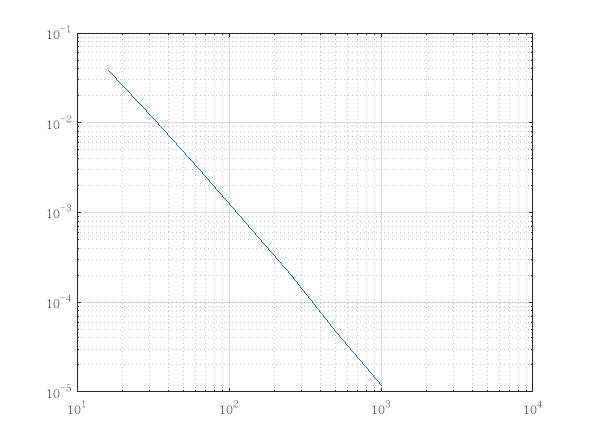
\includegraphics[scale=0.7]{pictures/p1_4_3.png}
      \caption{\small{三次样条插值(边界条件3)的最大误差随区间数$n$的变化}} %图2
    \end{figure}

    \par
    边界条件3和边界条件2的代码大同小异,就是要注意两者的线性方程组中的矩阵$A,M,d$都略不一样.这里我列出了计算边界条件3的矩阵$A,M,d$的代码:
    \begin{lstlisting}[frame=single]
% for boundary condition 3,
% get d(0) and d(n)
m_0 = 0;
m_n = 0;
    
d = d.';
d_0 = 6 * ( df(1) + df(n) );
d_n = 6 * (m_n - df(n) / h(n) ) / h(n);
d = [d_0; d];

% A is the parameters of this linear equation
% get A
A = 2 * eye(n);
A(1,1) = 2 * ( h(1) + h(n) );
A(1,2) = h(1);
A(1,n) = h(n);
A(n,1) = lambda(n-1);
A(n,n - 1) = mu(n-1);
for i = 2 : n - 1
    A(i,i-1) = mu(i);
    A(i,i+1) = lambda(i);
end
    \end{lstlisting}
    \end{itemize}
    
\item[第二题] \textbf{Newton插值法}

\begin{itemize}
  \item [(a)] \textbf{证明题} 
  \par
  由性质1.1可知,$k$阶差商
  \begin{equation}
    \begin{aligned}
    F[x_0,x_1, \cdots,x_k] = \sum_{i=0}^k 
    \frac{f(x_i)}{(x_i - x_0)\cdots(x_i - x_{i-1})\cdots(x_i - x_{i+1}) \cdots (x_i - x_k)}
    \end{aligned}
  \end{equation}

  \par
  由于$\{i_0,i_1, \cdots i_k\}$ 为 $\{ 0,1, \cdots k\}$的任一排列,
  因此$F[x_{i_0},x_{i_1}, \cdots,x_{i_k}]$只是改变了(11)式的求和次序,其结果不变.
  \par
  所以,$F[x_0,x_1, \cdots,x_k] = F[x_{i_0},x_{i_1}, \cdots,x_{i_k}]$.

  \item [(b)] \textbf{Newton插值(顺序选取插值点)的最大误差随插值点数的变化}
  \par 
  在这里,取 $ n = \{ 2^2, 2^3, 2^4, 2^5, 2^6, 2^7 \}$,
  分别从右到左选取插值点通过$n+1$个Chebyshev点对[-1,1]上的Runge函数进行插值,
  并取[-1,1]上2000个等距区间进行误差计算,得到最大误差随插值点数$n$的变化如图5所示.
  \begin{figure}[htbp]
    \centering
    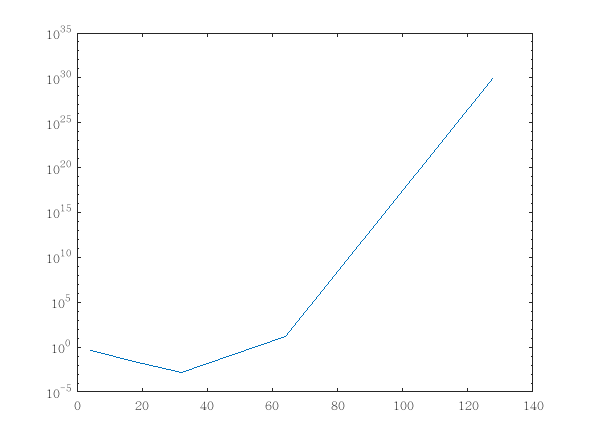
\includegraphics[scale=0.7]{pictures/p2_2.png}
    \caption{\small{顺序选取插值点进行Newton插值时,最大误差随插值点数$n$的变化}} %图5
  \end{figure}

  \item [(c)] \textbf{Newton插值(随机选取插值点)的最大误差随插值点数的变化}
  \par 
  在这里,取 $ n = \{ 2^2, 2^3, 2^4, 2^5, 2^6, 2^7 \}$,
  分别随机化选取插值点通过$n+1$个Chebyshev点对[-1,1]上的Runge函数进行插值,
  并取[-1,1]上2000个等距区间进行误差计算,得到最大误差随插值点数$n$的变化如图6所示.
  \begin{figure}[htbp]
    \centering
    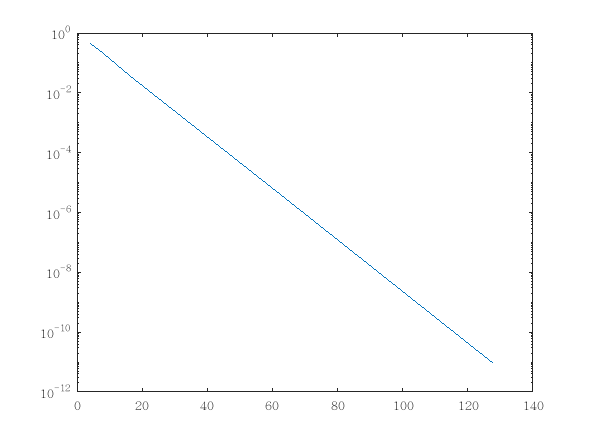
\includegraphics[scale=0.7]{pictures/p2_3.png}
    \caption{\small{随机选取插值点进行Newton插值时,最大误差随插值点数$n$的变化}} %图6
  \end{figure}

  \par
  这里,我的Newton插值的MATLAB代码如下所示;
  \begin{lstlisting}[frame=single]
% use Newton interpolation to approximate a function
% @F: the function to approximate in [-1,1]
% @n_list: stores the number of points to be inserted
% @k: number of testing points in [-1,1]
% @rand: whether to randomly choose the sequence of
%   interpolation points(1) or not(0).
% plot the semilogy of max error on each n in n_list
function Newton_interpolation(F, n_list, k,rand)

    % max_errors stores the max error 
    % of testing points on each n
    [~,n_list_col] = size(n_list);
    max_errors = zeros(1,n_list_col);
    
    % get the max_error on each n
    for index = 1 : n_list_col
        
        n = n_list(index);
        % get the sequence of interpolation points
        % { ( x(i),f(x(i)) ) }
        if(rand == 1)
            rng(22);
            x0 = randperm(n + 1);
            x0 = x0 - 1;
            x0 = x0 *(pi/n);
        else
            x0 = linspace(0, pi, n + 1);
        end
        x = cos(x0);
        f = F(x);
    
        % u is the list of testing points
        u = linspace(-1, 1, k);
        % fu is the exact function value
        % of each testing points
        fu = F(u);
        % Nu is the approximation function value
        % of each testing points
        Nu = u;
         
        % g is difference of each order
        g = f;
        for i = 2 : n + 1
            for j = n + 1 : -1: i
                g(j) = (g(j) - g(j-1)) ...
                        / (x(j) - x(j-i+1)); 
            end
        end
        
        % get the approximate value of each testing point
        for i = 1 : k
            % init the parameter t 
            % and interpolation value newton
            t = 1;
            newton = g(1);
            for j = 2 : n + 1
                t = t * ( u(i) - x(j-1) );
                newton = newton + t * g(j); 
            end
            Nu(i) = newton;
        end
        max_errors(index) = max( abs(fu - Nu) );
    end
    
    semilogy(n_list,max_errors);
end

  \end{lstlisting}

  \item [(d)] \textbf{解释上两问不同现象的原因}
  \par
  在(b)中,顺序选取插值点,在$n = 2^5$之前,最大误差都是随着$n$的指数增加而指数减小,但是当$n \geq 2^6$之后,最大误差却随着$n$的指数增加而大幅度增加. 当$n = 2^7$时,最大误差甚至达到了$2^30$的数量级.
  \par
  在(c)中,随机选取插值点,最大误差都是随着$n$的指数增加而指数减小.
  \par
  原因: 可能是顺序选取插值点时,MATLAB存在精度溢出,导致一个本来很小的数变成了一个很大的数.而随机选取插值点时,MATLAB避免了精度溢出.
\end{itemize}

\item[第三题] \textbf{Lagrange插值法}
  
    \begin{itemize}
      \item [(a)] \textbf{证明$l_k(x_j) = \delta_{k,j}$} 
      \par
      当$n$为奇数时,有
      \begin{equation}
        \begin{aligned}
          $l_k(x_j) = \frac{(-1)^k}{n} \frac{sin(n \pi x_j)} {sin(\pi(x_j - x_k))}$
        \end{aligned}
      \end{equation}
      
      \par
      若$ j \neq k$,则有$x_j - x_k = \frac{j-k}{n}$,其中$0 < j - k < n$.
      因此$sin(\pi(x_j - x_k)) = sin(\frac{(j-k)\pi}{n}) \neq 0$,
      并且$sin(n\pi x_j) = sin(j\pi) = 0$.
      所以此时$l_k(x_j) = 0$.

      \par
      若$ j \to k$,则由洛必达法则,有
      $ \lim\limits_{j \to k} l_k(x_j) = 
      \lim\limits_{j \to k} \frac{(-1)^k}{n} \frac{sin(n \pi x_j)} {sin(\pi(x_j - x_k))} \\ = 
      \lim\limits_{j \to k} \frac{(-1)^k}{n} \frac{n\pi cos(n \pi x_j)} {\pi cos(\pi(x_j - x_k))} = 
      (-1)^k cos(k \pi) = 1 $
      

      \par
      同理,当$n$为偶数时,有
      \begin{equation}
        \begin{aligned}
          $l_k(x_j) = \frac{(-1)^k}{n} \frac{sin(n \pi x_j)cos(\pi(x_j - x_k))} {sin(\pi(x_j - x_k))}$
        \end{aligned}
      \end{equation}
      
      \par
      若$ j \neq k$,则有$x_j - x_k = \frac{j-k}{n}$,其中$0 < j - k < n$.
      因此$sin(\pi(x_j - x_k)) = sin(\frac{(j-k)\pi}{n}) \neq 0$,
      并且$sin(n\pi x_j) = sin(j\pi) = 0$.
      所以此时$l_k(x_j) = 0$.

      \par
      若$ j \to k$,则由洛必达法则,有
      $ \lim\limits_{j \to k} l_k(x_j) = 
      \lim\limits_{j \to k} \frac{(-1)^k}{n} \frac{sin(n \pi x_j)} {sin(\pi(x_j - x_k))} \\ = 
      \lim\limits_{j \to k} \frac{(-1)^k}{n} \frac{n\pi cos(n \pi x_j)cos(\pi(x_j - x_k)) - \pi sin(n\pi x_j)sin(\pi (x_j - x_k))} {\pi cos(\pi(x_j - x_k))} = 
      (-1)^k cos(k \pi) = 1 $

      \par
      因此,无论$n$为奇数还是偶数,都有$l_k(x_j) = \delta_{k,j}$.

      \item [(b)] \textbf{插值误差随$x$的变化} 
      \par
      使用$[0,1]$上不等距的$n = 2^6$个点,基于给定的插值基函数,对$f(x)$进行Lagrange插值.并取$[0,1]$上等距的$1000$个点进行误差计算,得到了这$1000$个点的逐点误差如图7所示.
      \begin{figure}[htbp]
        \centering
        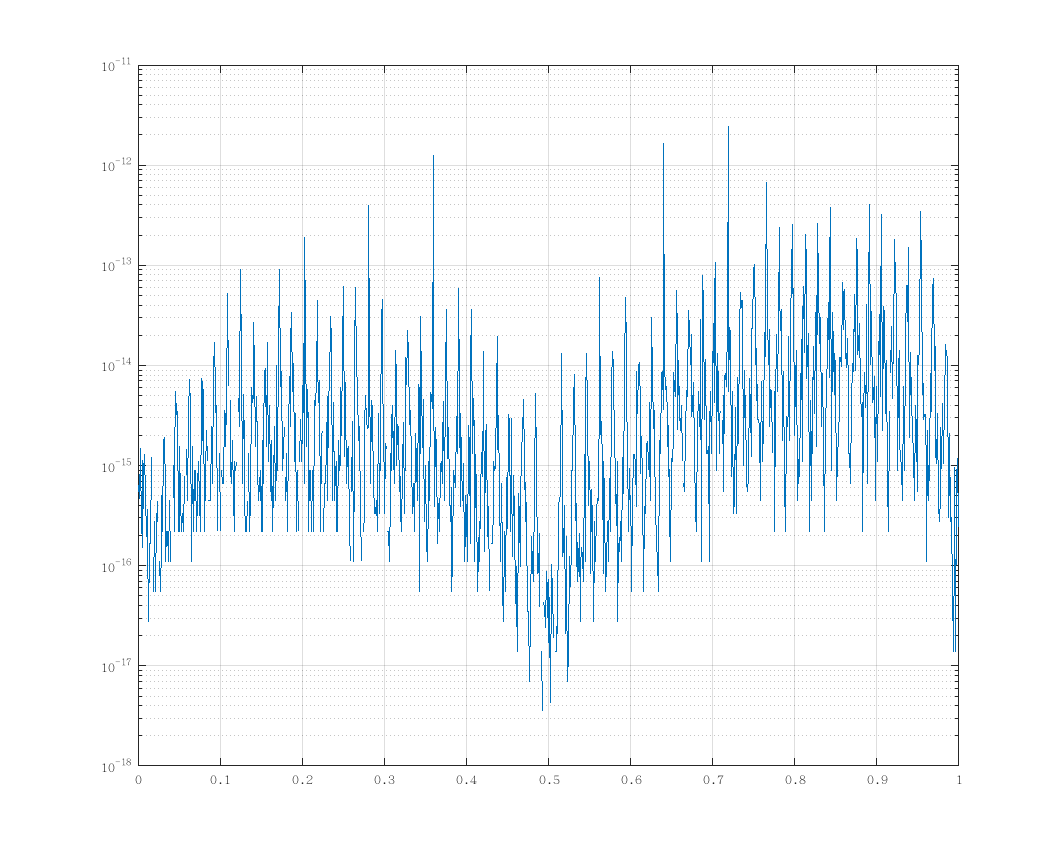
\includegraphics[scale=0.7]{pictures/p3.png}
        \caption{\small{Lagrange插值误差随$x$的变化}} %图7
      \end{figure}

      \par
      而实现该算法的MATLAB代码如下所示.
    \begin{lstlisting}[frame=single]
% use Lagrange interpolation to approximate a function
% @F: the function to approximate in [-1,1]
% @L_k_odd: the base function when n is odd
% @L_k_even: the base function when n is even
% @n: number of interpolation points
% @k: number of testing points in [0,1]
% plot the semilogy of errors
function Lagrange_interpolation(F,L_k_odd, L_k_even, n, k)

    % get the sequence of interpolation points
    x = linspace(0, 1, n);
    
    % select base function
    if( mod(n,2) == 1)
        l = L_k_odd;
    else
        l = L_k_even;
    end
    
    % get the testing points
    test_x = linspace(0,1,k);
    % the actual function value of testing points
    f = F(test_x);
    % the evaluated function value of testing points
    L = zeros(1,k);
    
    % get the error of each testing point
    for i = 1 : k
        tmp = 0;
        % sum on each interpolation point
        for j = 1 : n
            tmp = tmp + l(test_x(i), j, n) * f(i);
        end
        L(i) = tmp;
    end
    % get the errors on each testing point and plot them
    error = abs(L-f);
    semilogy(test_x,error);
    grid on;
end
    \end{lstlisting}

    \end{itemize}

\item[第四题] \textbf{最小二乘法}
  \begin{itemize}
  \par
  我们尽量使用多项式函数来拟合.
  然而,题目中所给的$f(x) = \frac{x}{a+bx}$并不是多项式.
  所以,我们需要对输入数据进行预处理.
  令$\hat{y} = \frac{1}{y}$,$\hat{x} = \frac{1}{x}$,
  则由$y = \frac{x}{a+bx}$得$\frac{1}{y} = \frac{a}{x} + b$,
  即$\hat{y} = a\hat{x} + b$.
  然后,再求解法方程,即可得到$a = 2.486700,b = 0.462251$,
  拟合函数为$f(x) = \frac{x}{2.486700 + 0.462251x}$,拟合函数对比所给数据点的2-范数为$0.005978$,拟合函数和所给数据点的图像如图8所示,MATLAB代码如下:
  \begin{lstlisting}[frame=single]
% x-value of four original input points 
X = [2.1, 2.5, 2.8, 3.2];
% y-value of four original input points
Y = [0.6087, 0.6849, 0.7368, 0.8111];

% preprocess the data to fit in linear LSM
% now y = x / (a + bx) <=> y_inv = a*x_inv + b
X_inv = 1 ./ X;
Y_inv = 1 ./ Y;

alpha = Least_square_method(X_inv,Y_inv);

a = alpha(2);
b = alpha(1);

% The approximate function
syms x;
F = @(x) x ./ (a + b .* x);

% get the 2-norm of error on each points
Y_appro = F(X);
errors = Y - Y_appro;
err = norm(errors,2);
% print a,b,err 
fprintf('Approximate f(x) = x / (%10.6f +%10.6f x )\n',a,b);
fprintf('The 2-norm of errors is %10.6f\n',err);

% plot the approximation function
x= 2 : 0.01 :4;
y = F(x);
scatter(X,Y,'k*');
hold on;
plot(x,y);

% implement Least_square_method
% to get a linear approximate function Y = aX + b
% @X: x-value of input points 
% @Y: y-value of input points
% return the coeffient vector alpha
function alpha = Least_square_method(X,Y)
    % coefficients of linear function
    alpha = zeros(2,1);
    % number of input points
    n = length(X);
    % A stores different order of xi
    A = ones(n,2);
    for i = 1 : n
        A(i,2) = X(i);
    end
    
    % A^T * A * alpha = A^T * Y^T
    % that is, L * alpha = R
    L = A.' * A;
    R = A.' * Y.';
    alpha = L \ R;
end
  \end{lstlisting}

  \begin{figure}[htbp]
    \centering
    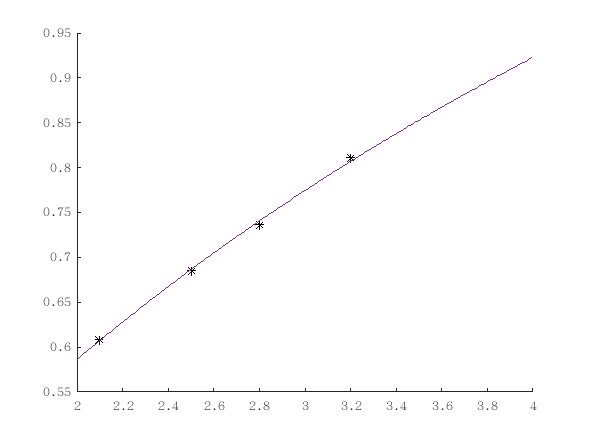
\includegraphics[scale=0.7]{pictures/p4.png}
    \caption{\small{拟合函数和所给数据点}} %图8
  \end{figure}
  \end{itemize}
\end{enumerate}

\end{document}